\documentclass[12pt,letterpaper]{article}
\usepackage[latin1]{inputenc}
\usepackage{amsmath}
\usepackage{amsfonts}
\usepackage{amssymb}
\usepackage{setspace}
\usepackage{graphicx}
\usepackage{epsfig}
\graphicspath{{./images/}} % Figures path - used in graphicx
\author{Christopher C. Lamb}
\title{Policy Overlay Networks}
\date{\today}
\begin{document}

\maketitle

\doublespacing

\begin{abstract}
Abstract - TBD
\end{abstract}

\section{Introduction}
Current enterprise computing systems are facing a troubling future.  As things stand today, they are too expensive, unreliable, and information dissemination procedures are just too slow.

Generally, such systems still do not use current commercial resources as well as they could and use costly data partitioning schemes.  Most of these kinds of systems use some combination of systems managed in house by the enterprise itself rather than exploiting lower cost cloud-enabled services.  Furthermore, many of these systems have large maintenance loads imposed on them as a result of internal infrastructural requirements like data and database management or systems administration.  In many cases networks containing sensitive data are separated from other internal networks to enhance data security at the expense of productivity, leading to decreased working efficiencies and increased costs.

These kinds of large distributed systems suffer from a lack of stability and reliability as a direct result of their inflated provisioning and support costs.  Simply put, they large cost and effort burden of these systems precludes the ability to implement the appropriate redundancy and fault tolerance in any but the absolutely most critical systems.  Justifying the costs associated with standard reliability practices like diverse entry or geographically separated hot spares is more and more difficult to do unless forced by draconian legal policy or similarly dire business conditions.

Finally, the length of time between when a sensitive document or other type of data artifact is requested and when it can be delivered to a requester with acceptable need to view that artifact is prohibitively long.  These kinds of sensitive artifacts, usually maintained on partitioned networks or systems, require large amounts of review by specially trained reviewers prior to release to data requesters.  In cases where acquisition of this data is under heaving time constraints like sudden market shifts or other unexpected conditional changes this long review time can result in consequences ranging from financial losses to loss of life.

Federal computer systems are prime examples of these kinds of problematic distributed systems, and demonstrate the difficulty inherent in implementing new technical solutions.  They, like other similar systems, need to be re-imagined to take advantage of radical market shifts in computational provisioning.
\section{Motivation}
Current policy-centric systems are being forced to move to cloud environments and build much more open systems.  Some of these environments will be private or hybrid cloud systems, where private clouds are infrastructure that is completely run and operated by an organization for wider use and provisioning, while hybrid clouds are combinations of private and public cloud systems.  Driven by both cost savings and efficiency requirements, this migration will result in a loss of control of computing resources by involved organizations as they attempt to exploit economies of scale and utility computing.

Robust usage management will become an even more important issue in these environments.  Federal organizations poised to benefit from this migration include agencies like the National Security Agency (NSA) and the Department of Defense (DoD), both of whom have large installed bases of compartmentalized and classified data.  The DoD realizes the scope of this effort, understanding that such technical change must incorporate effectively sharing needed data with other federal agencies, foreign governments, and international organizations \cite{proposal:info-sharing-strategy}.  Likewise, the NSA is focused on exploiting cloud-centric systems to facilitate information dissemination and sharing \cite{proposal:nsa-cloud}.

Cloud systems certainly exhibit economic incentives for use, providing cost savings and flexibility but they also have distinct disadvantages as well.  Specifically, the are not intrinsically as private as some current systems, generally can be less secure than department-level solutions, and have the kind of trust issues that therapists cannot adequately address \cite{proposal:privacy-security-trust-cloud}.

To begin with, cloud technology is not currently as private as some organizations would like:
\begin{itemize}
\item \textit{User Data Control} --- In virtually any given Software-as-a-Service (SaaS) scenario, user data controls are sadly lacking.  Once data has been committed to a specific provider, that data is completely out of the original data owners control.  Furthermore, as we will see below, that data my not even be solely owned by the original owner anymore either.
\item \textit{Secondary Use} --- Most consumer facing social systems extensively mine user provided data for additional business advantages.  This is a common and well known secondary use for supplied data.  SaaS providers again have strong incentives to examine user provided information.
\item \textit{Offshore Development} --- Service users have no real control over who actually develops the systems a given service deploys.  Organizations have attempted to contractually limit development and support functions companies pursue to, say, the continental United States but have had very poor results with these kinds of unsupportable arrangements.
\item \textit{Data Routing} --- System providers in fact have little control over routing issues as well as system users.  Prohibiting data routing through sensitive countries is a difficult task for a single organization.
\item \textit{Secondary Storage} --- Most large-scale systems expect to use Content Delivery Networks (CDNs) to help manage content, and that expectation is heavily reflected in their physical system architectures. They simply cannot divorce use of CDNs from their systems for a single organization.
\item \textit{Bankruptcy and Data Ownership} --- Ownership and obligation to maintain expected data arrangements for a given company is unestablished under bankruptcy \cite{proposal:borders-info-I,proposal:borders-info-II,proposal:borders-info-III}.
\end{itemize}

Security issues also emerge from utility computing infrastructures:
\begin{itemize}
\item \textit{Data Access} --- System users have very little control over who, in the system provider's organization, is able to access their data and systems.
\item \textit{Data Deletion} --- Most savvy organizations have procedures in place to sanitize old storage elements like disk drives or backup tapes.  System users have very little control over if and how this is done when computing services are treated as a utility.
\item \textit{Backup Data Storage} --- Backup media is very difficult to encrypt, and most system providers still use tape systems as preferred media solutions for backup and storage needs.  These tapes, or copies of them, are generally stored offsite to support disaster recovery scenarios.  Security of these types of systems has been spotty to date \cite{proposal:saic-breach-I,proposal:saic-breach-II,proposal:saic-breach-III}.
\item \textit{Intercloud Standardization} --- Cloud computing systems do not have any standardized way to transfer computational units or data between systems.  Any protocols used for this kind of thing must be developed by customers themselves.  Due to the desire of providers to lock-in customers, this will likely not change as any standard development is strongly counter-incentiveized. 
\item \textit{Multi-tenancy and Side-Channels} --- Multi-tenant architectures in which multiple customers simultaneously use the same systems open those customers to covert side-channel attacks.
\item \textit{Logging and Auditing} --- Logging and auditing structures, especially for inter-cloud systems, are non-existent.
\end{itemize}

Finally, such systems suffer from internal and external trust issues:
\begin{itemize}
\item \textit{Trust Relationships} --- Trust is difficult to establish between individual cloud providers long-term.
\item \textit{Consumer Trust} --- Service users are still not entirely trusting of cloud system providers.
\end{itemize}

How to address these issues is an open research question.  Organizations ranging from cloud service providers to the military are exploring how to engineer solutions to these problems, and to more clearly understand the trade-offs required between selected system architectures \cite{proposal:assured-info-sharing}.  The problems themselves are wide ranging, appearing in a variety of different systems.  Military and other government systems are clearly impacted by these kinds of trust and security issues, and they also have clear information sensitivity semantics.  This, coupled with the fact that these organizations have been dealing with these issues in one form or another for decades make them very well suited for prototypical implementation and study.

The current standard in place dealing with these issues in this environment is managed by the Unified Cross Domain Management Office (UCDMO).  UCDMO stakeholders range from the DoD to the NSA.  The current standard in place and governed by the UCDMO to deal with this kinds of issues are \textit{guard-centric cross domain architectures}.

\subsection{Current Solutions}
Current and near-future proposed solutions endorsed by the UCDMO include system architectures assembled by the NSA, Raytheon, and Booz Allen Hamilton (BAH).   The NSA has been active in this area for decades as a logical extension of their role in signals intelligence collection and processing.  Raytheon and BAH have been engaged over the past few years to provide an alternative voice and design approach to these kinds of systems, an effort met with limited success.

These cross-domain solutions are intended to enable sensitive information to easily flow both from a higher sensitivity domain to a lower sensitivity domain, and from lower to higher as well.  They generally act over both primary data (say, a document) and metadata over that primary data as well.  Note that in these system, in most cases, human intervention is still required to adequately review data prior to passing into lower security domains.

\subsubsection{NSA, Filtered}
The NSA conducted initial work in this area.  Their standard-setting efforts culminated in a reasonable conceptual system architecture, using groups of filters dedicated to specific delineated tasks to process senistive information \cite{proposal:nsa-arch}.
\begin{figure}[!t]
\centering
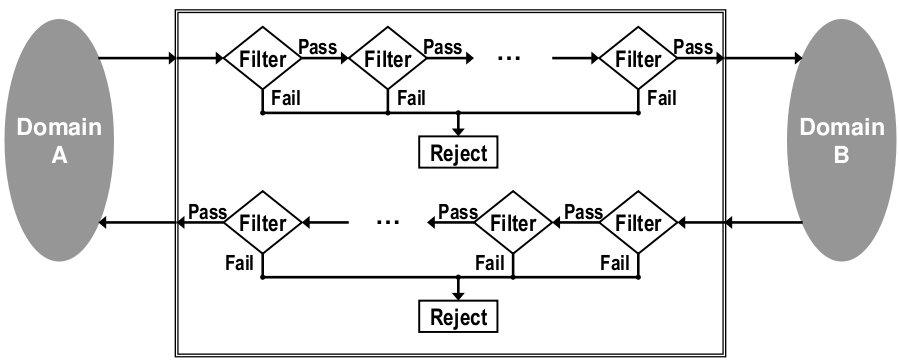
\includegraphics[width=5in]{nsa-legacy-arch}
\caption{NSA Legacy Notional Architecture Model}
\label{fig:model:conceptual-model}
\end{figure}

\subsubsection{NSA, Services}

\subsubsection{Raytheon}

\subsubsection{Booz Allen Hamilton}



\section{Related Work}

\section{System Architecture}

\section{Conclusions}

\bibliographystyle{plain}
\bibliography{bib/proposal}

\end{document}